\section{Definición de requisitos y análisis}
\label{sec:definicion_de_requisitos_y_analisis}

\subsection{Definición de requisitos}

A continuación se enumeran los requisitos para el desarrollo del trabajo:

\begin{itemize}
	\item Implementar y entrenar una red neuronal que genere un modelo capaz de detectar baches en el asfalto a partir de imágenes
	\item El modelo deberá ser capaz de procesar una imagen en un tiempo lo más cercano posible a 1/30s, para ser capaz de procesar video en tiempo real
	\item El modelo deberá poderse ejecutar en un dispositivo móvil Android
	\item El modelo será alimentado directamente con la salida de la cámara del dispositivo móvil
\end{itemize}

\subsection{Arquitectura}

\begin{figure}[H]
	\centering
	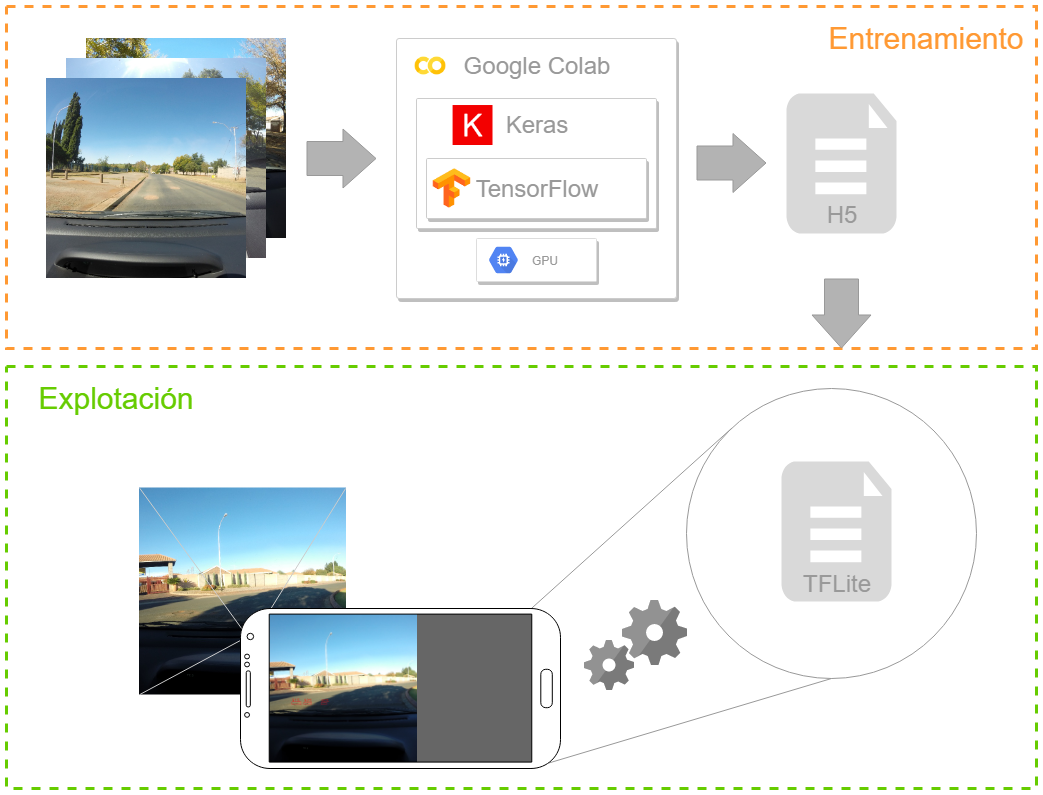
\includegraphics[width=\linewidth]{images/architecture.png}
	\caption{Arquitectura}
	\label{fig:architecture}
\end{figure}

Como se puede observar en la figura \ref{fig:architecture}, la arquitectura está dividida en dos partes. Una parte se utiliza para entrenar la red neuronal y generar el modelo. La otra parte se utiliza para explotar el modelo generado.

El entrenamiento de la red neuronal requiere de una infraestructura con un hardware potente, que incluya GPU para reducir los tiempos de entrenamiento. Sin embargo la explotación del modelo generado, no  requiere de un hardware potente, y puede ejecutarse directamente en un dispositivo móvil en posesión del usuario final. El modelo obtenido después de la fase de entrenamiento requiere de una transformación a un formato concebido para ser ejecutado en dispositivos con recursos limitados.

\subsection{Tecnologías}

Todo el proyecto ha sido desarrollado utilizando Python, a excepción de la aplicación Android, que ha sido desarrollada en Java.

Para todo lo relacionado con el tratamiento de imágenes se ha utilizado el paquete de python OpenCV. Este tratamiento incluye la lectura de imágenes, recorte, reescalado y volteo de las imágenes, visualización de las predicciones obtenidas, etc.

Para la implementación de la red neuronal se ha utilizado Keras, que es un envoltorio sobre Tensorflow que simplifica su uso. Dada una arquitectura de red neuronal, con Keras es muy sencillo definir las capas y sus interconexiones. Además Keras proporciona clases que facilitan la definición de un conjunto de imágenes como entrada de la red neuronal. Keras también proporciona una serie de eventos con la idea de poder suscribirse a los mismos y poder reaccionar en consecuencia, como por ejemplo, suscribirse al evento de final de época y salvar el modelo si este ha mejorado con respecto a la época anterior.

Después de realizar un estudio del estado del arte en la resolución de problemas de detección de objetos y con los requisitos definidos para el proyecto, se ha decidido optar por la utilización de YOLO para el desarrollo del mismo. Concretamente se van a utilizar dos versiones de YOLO: \textit{YOLO V3 Tiny}, diseñada para ejecutarse en dispositivos con recursos limitados y \textit{YOLO V3}, para compararla con la anterior. El proyecto se basa en un par de implementaciones de YOLO para Keras \cite{s3_yolov3_orig} \cite{s3_yolov3tiny_orig}. Se han unido ambas implementaciones en una única \cite{s3_yolo_dicastro} que soporta ambas versiones de YOLO. Además, se han realizado múltiples desarrollos complementarios para mejorar la funcionalidad, como por ejemplo, adición de soporte en formato txt para el etiquetado de las imágenes y adición de nuevos parámetros de configuración para mejorar el resultado del entrenamiento.

Para la ejecución de los modelos obtenidos en un dispositivo móvil de ha utilizado TFLite. Este paquete permite transformar distintos tipos de modelo (keras, tensorflow) a formato TFLite y ejecutar estos modelos en dispositivos con recursos reducidos. En las últimas versiones de esta librería se soporta, aunque de forma experimental, el uso de la GPU del dispositivo.

La aplicación móvil ha sido desarrollada en java para la plataforma Android. Se ha hecho uso de la librería de TFLite, disponible para java, que hace que la carga y ejecución del modelo sea una tarea trivial.